\def\stmt{$A$}
% \def\stmt{$\phi$}


\commentout{%oli-v1
	% The ability articulate a \emph{degree of confidence} is an important aspect of knowledge representation.
	The ability to articulate a \emph{degree of confidence} 
	% (or the opposite: a degree of uncertainty)
	is a critical aspect of representing knowledge.
	There are 
	% Correspondingly, there are
	many well-established ways to quantify (un)certinaty \parencite[\S2]{halpern2017reasoning},
		and chief among them is probability.
	While ``confidence'' can be coherently read in probabilistic terms,
		such usage may shadow another important concept.
	This paper details a different conception that arises when updating beliefs. 
	As we shall see, this notion of confidence
	complements traditional representations of uncertainty (such as probability), 
	and moreover unifies several different concepts across AI.
}

What should it mean to say that one has a high degree of confidence in a statement $\phi$?  It is often taken to mean that we think $\phi$ is likely. 
% This paper details a different conception that arises when updating beliefs. 
% As we shall see, this notion of confidence
% complements traditional representations of uncertainty (such as probability), 
Here we argue that there is a related but more useful conception of confidence that arises when updating---one that complements likelihood and, moreover, unifies several different concepts in the literature.
% Here we argue that there is a related but more useful way of defining confidence, which complements notions like probability and, moreover, unifies several different concepts in the literature.

% For us, confidence is a measure of trust (in incoming information), rather than of likelihood (of hypothetical information). 
% For us, confidence (in an input $\phi$) is a measure of \emph{trust}, rather than of likelihood; it quantifies seriously to take $\phi$ in updating one's beliefs.
%
%joe1:
% For us, the degree of confidence in $\phi$ is a measure of the degree
% to which we \emph{trust} $\phi$,
% rather than of the likelihood of $\phi$.  We formalize this by taking
% the degree of confidence to represent how seriously to take $\phi$
% when updating beliefs.
%
%oli1: with reference to your rewrite (above): I don't like the way the grammar 
% worked out; my lead-in "for us" muddies the "our confidence" part 
% that you wrote. Let me try to clean it up. 
%
For us, confidence is a measure of \emph{trust}, rather than likelihood.
In particular, the {degree of confidence} that one has in a piece of information $\phi$
%is a number  $\chi \in [\bot,\top]$ that 
quantifies how seriously to take $\phi$ in updating one's beliefs. 
%oli1:
% In the below, I replaced "0" and "1" with "no" and "full" because
% I want don't want to lock in the range [0,1] at this level of generality.
% More importantly, the second part about "taking \phi to be true" doesn't
% make as much sense in general, so I rephrased it.
%
% Thus, if we learn $\phi$ but have confidence 0 in it, it should not
% affect our beliefs at all, while if we have confidence 1 in $\phi$, we
% should update our beliefs by taking $\phi$ to be true; in a
% probabilistic setting, this amounts to conditioning on $\phi$. 
%
% Thus,
So at one extreme,
if we observe $\phi$ but have no confidence in it, 
% it should not affect our beliefs at all;
we should not change our beliefs at all;
at the other, if we have full confidence in $\phi$,
 we should fully incorporate it into our beliefs.
 
% , in some sense.
% In the setting where, our beliefs is a probability measure $\Pr$, and $\phi$ is an event, 
% In a probabilistic setting, we can capture an intermediate degree of
% If our belief state is a probability measure $\Pr$ and $\phi$ is an event, for example, then fully incorporating $\phi$ amounts to conditioning $\Pr$ on it.
\begin{example} \label{ex:prob-simple}
% Suppose, for example, that 
Suppose
% For example, if
our belief state is a probability measure, and $\phi$ is an event. 
% In this setting, 
% Here,
A full-confidence update then amounts to conditioning on $\phi$, after which $\phi$ has probability 1, and so cannot be further incorporated.
%oli1: changed from "the obvious way" to "an obvious way"
% In a probabilistic setting, we can capture an  intermediate degree of confidence by interpolating in the obvious way:
% In this case,
% we can also capture intermediate degrees of confidence in an obvious way:
We also have an obvious way to describe intermediate degrees of confidence:
if we learn $\phi$ with confidence
%oli1: now adding range here
% $\alpha$
$\alpha \in [0,1]$
% and start with a prior probability $\Pr$, then we end up with the
and start with prior probability $\Pr$, then we end up with the
%oli1: I agree that this notation is nicer, but these days it
% is also much less standard than p(X) and p(X|\phi). In particular,
% my ML friends who work with applied probability a lot do not understand
% how to parse  "\Pr | \phi". 
posterior $(1-\alpha)\Pr + \alpha (\Pr\mid \phi)$.
%
Thus, having high confidence in $\phi$ leads to posterior beliefs that give $\phi$
high
%oli1: I've seen a lot of statistics people make a big fuss about
% this being the wrong usage of the word "likelihood", which I've been
% told applies to evidence that is being conditioned on, and not to 
% events whose probability we're querying.  Now that we have a
% probability in scope, I'd prefer to avoid this fight by just saying:
%likelihood.
probability.
% But confidence and probability are not always so tightly coupled.
% Still, confidence and probability are quite different in general.
The converse is false, however, so
confidence and probability can still be quite different.
% 
%oli1: the context here has been stripped; we're now missing how it might be possible to learn \phi with low confidence if we already assign it high probability.
% If we start out with a prior that gives $\phi$ high likelihood, and learn $\phi$ with low confidence, our posterior beliefs still give $\phi$ high likelihood.  
% We might also have a great deal of confidence in an observation of $\phi$  despite having a low prior belief in $\phi$.
If an untrusted source tells us $\phi$ which we already happen to believe, 
then our prior assigns $\phi$ high probability,
we learn $\phi$ with low confidence,
and then our posterior beliefs still give $\phi$ high probability.  
% Confidence is even easier to distinguish from prior probability: 
Confidence and prior probability are even more independent: 
if we learn a surprising fact $\phi$ from a trusted source, we have high confidence in $\phi$ despite it having low prior probability.
% This leads to an important observation: one's confidence in $\phi$ is not a feature of one's prior probability at all.
\end{example}

\commentout{
	In this context, 
	the confidence $\chi \in [0,1]$ has a clear interpretation as the ``fraction of the way towards full incorporation'',
	but in others,
	it may be 
	less clear what a number on this scale (say, $\chi{=}0.7$) means.
	% there is still a natural path from distrust to complete trust that is parameterized differently.
	% In other cases, there are other more natural ways to articulate one's confidence.
}

%oli1: something bothers me about starting a paragraph with "but", 
% especially without directly pushing off of something concrete about the
% way the previous sentence ended.
% But confidence can be applied far more broadly.
% This notion of confidence applies far more broadly. 
This notion of confidence applies far more broadly.
% Here is an example that has similar 
% We now give a quite different ,
We now give an example with the same critical elements,
but a very different flavor.
% of a very different flavor, 
% in which confidence is measured differently.

\begin{example}\label{ex:classifier}
Consider a neural network, whose ``belief state'' is a setting of weights.
% $ \in \mathbb R^n$.
	% which are updated when given a training point.
% As it sees each training point, it updates its weights. 
% Modern learning algorithms do not take any individual point too seriously; each training point $x$ changes the weights incrementally, and alone may not even be enough for the network to classify that point correctly.
%oli1:adding, per our discussion
For definiteness, suppose we are talking about a classifier, so that for every setting of weights $\theta$, there is a function
%oli1: I can also siplify this to be a function f : X \to [0,1] if it's
% a binary classifier, which will simplify the text. 
$f_\theta : X \to \Delta Y$ that maps inputs $x \in X$ to distributions $f_\theta(x)$ over possible class lables $Y$. 
%joe1*: You're going on a long digression here that's irrelevant.
%This is the opposite of "clean and crisp".  Just cut to the chase:
%what does confidence mean in this setting? What is it that gets
%confidence?  This is not the least bit clear to me from your
%writeup.  You say that we can quantify confidence by the number of
%training iterations, but I don't see how to relate that to having a
%high degree of confidence in \phi.  What's \phi?
%oli1*: what I said was all relevant and curated, but evidently it wasn't
% clear and I lost you pretty early on. I'm trying to fill out what I had
% so it's easier to follow.
Modern learning algorithms (like gradient descent) make small incremental changes to the weights.
Therefore, if we update $\theta$ with a labeled training example $\phi = (x,y)$ to obtain new weights $\theta'$, there is no guarantee that $f_{\theta'}(x)$ gives high probability to $y$---only that it will be higher than it was before.
 % that it assigns higher probability to $y$ than $f_{\theta}(x)$ does. 
% does not guarantee that the resulting network handles $x$ correctly. 
% In other words, the algorithm does not take any individual point too seriously.
In other words, such algorithms 
(in contrast to their historical counterparts like conjunction learning algorithms \parencite{conjunctions}) 
do not take any one encounter with a training example too seriously---
%oli1:added
\unskip that is, they make low-confidence updates. 
% So, in contrast with conditioning, there is a significant difference betwen cycling through the training data once, and doing so many times.
This relative distrust of each individual sample is arguably what makes the training process robust to noisy or contradictory observations.
\commentout{
	As a result,
	there is a significant difference between going through the training data once
	 % (a single epoch)
	\unskip, and doing so many times.}
%oli1: paragraph break now that we have example structure to hold it together

Nevertheless, 
% the weights do eventually converge if we repeatedly train on $x$, 
if we train by repeatedly updating with the sample $\phi$, 
% which is a natural notion of 
% % ``fully incorporating $x$''---%
% full incorporation---%
the weights do eventually converge.%
	\footnote{Note for Joe: this is a white lie; the truth depends a bit on the architecture, and we may require that the space is compact. But this can be easily achieved by considering weights taking extended real values.}
% At the other extreme, if we had no trust in $x$, we could ignore it leaving our weights unchanged. 
% In this context, 
% Once again we have two extremes:
% Depending on our confidence, 
% How we ought to treat $x$ 
% What we ought to do depends on our confidence.
% At one extreme, we have no trust in $x$ and should ignore it, leaving weights unchanged; at the other, we trust $x$ completely, we should adopt the weights that arise in the limit of infinite training. 
% Moreover, this sequence of incremental updates (roughly) describes a path between the two extremes.%
%oli1: slowing down to fill out the story and explicitly bring out the connection to the other one
Doing so would be an extreme action, and only appropriate if we have complete trust in $\phi$, meaning we think important that $x$ always be classified as $y$.
At the opposite extreme, if we have no trust in $\phi$, we should simply discard it without changing our weights. 
Furthermore, our definition of a full-confidence update 
already suggests what to do for intermediate levels of confidence: simply stop the training process before convergence.
 % if we train with the sample $\phi$ but stop early,
Consequently, the number of training iterations $n$ 
functions as a description of 
% how to handle
intermediate levels of confidence: it interpolates
% the sequence of itermediate settings of weights 
%oli1: I'll save this verbage for later, per your request
% describes a path
% provides.
between no confidence (zero iterations) and full confidence (infinite iterations).
% \footnote{Another white lie: This path can be made into a continuous path by interpolating with a line segment, and made smooth in the limit of small step sizes; we will deal with both constructions in \cref{sec:project-additive}.}
% As we will see in \cref{sec:loss-repr}, such 
% We have now seen a new way of quantifying confidence: the number of training iterations.
% The number of training iterations a different way of quantifying confidence.  
% It turns out that in general, there are close relationships 
% \commentout{

	This way of measuring confidence also has a convenient property:
	% starting from intital weights $\theta$,
	first updating with confidence $n$ (that is, performing $n$ training iterations),
	and then afterwards updating with confidence $m$ (so $m$ additional iterations),
	is equivalent to a single update with confidence $m+n$.
	We call a measure of confidence that behaves this way \emph{additive}.
% }
\end{example}

% While there are some good reasons to prefer the first approach, 
% the second one is more general. 
%
%joe1: I have no idea what the "first" approach and the "second
%approach" are.  Is the second approach [0,\infty].  If so, this is
%the wrong place to discuss it.  It's a minor technical issue. 
%oli1*: you're right, what I wrote here was sloppy. However, I don't
% agree that this is a minor technical issue, because the point is
% to illustrate how one can measure confidence. I promise we will 
% not want to hide the [0,\infty] scale, because many of the concepts
% I plan on unifying under the word "confidence" are typically 
% measured in this scale. However, I will 
%
% We have now seen two very different descriptions of confidence. 
We have now seen two very different ways of describing confidence. 
% Which one should we prefer?
Are they related? 
Should we prefer one style over the other?
% Should we prefer one way of describing confidence over the other?
The number $\alpha \in [0,1]$ used in \cref{ex:prob-simple}
% \unskip, which we call \emph{fractional confidence}, 
appears to have an important advantage: an intermediate value can be clearly interpreted as a ``proportion of incorporation'', while the number of training iterations $n$ used in
\cref{ex:classifier} only really has meaning relative to
% the algorithm that performs the incremental updates.
% other values of $n$. 
other values of $n$ for the same training algorithm.
% the way in which individual updates are performed.
%
% But by the same token, the latter description turns out to be more general.
On the other hand,
% % the additive description in \cref{ex:classifier}
% the description in \cref{ex:classifier}
the apprach taken in the second example
appears to be more general. 
% But the approach used in the second example appears to be more general.
% The proportion of incorporation $\alpha \in [0,1]$ does 
	% make as much sense in \cref{ex:classifier},
It is not clear that a proportion $\alpha \in [0,1]$ 
is meaningful in \cref{ex:classifier},
but \cref{ex:prob-simple} can be
readily captured by a number of iterations 
% $n \in [0,\infty]$, as follows.
$n$, as follows.
% capture proportional confidence $\alpha \in [0,1]$ as follows.
% 
% For example, we can use the quantification of uncertainty from \cref{ex:classifier} to treat \cref{ex:prob-simple} as follows. 
%
%joe1: And I still object strongly to "unit of confidence". 
%oli1: I don't understand the objection. What I originally wrote
% needed (and may still needs) fixing, but I'm convinced that 
% this is an important part of how everything fits together. I've
% redone it below because I think it provides a very nice lead-in
% to Shafer's theory of evidence, and brings up some fundemental
% questions early.
%
If we fix some ``unit confidence'', say $\iota=0.01$,
then sequentially performing $n$ updates of confidence $\iota$ is 
equivalent to a single one of confidence $\alpha= 1-(0.99)^n$.
% Therefore, confidence $\alpha$ corresponds to a sequence of
% Therefore, 
% Or to say the same thing backwards:
Or, inverting:
to specify confidence $\alpha$, it suffices to 
instead give the number
% $t = \log (1 - \alpha ) / \log(1-\iota)$
\begin{equation} \label{eq:loglogiota}
 	n = \log (1 - \alpha ) / \log(1-\iota) 
	\quad\in[0,\infty]
\end{equation}
of confidence $\iota$ updates to be performed in sequence.
% A natural number describing the number of incremental updates (as in  \cref{ex:classifier}) is in some ways less satisfying then a number between zero and one (as in \cref{ex:prob-simple});
% In some ways, the way of describing confidence in \cref{ex:classifier}
% is less satisfying than that of \cref{ex:prob-simple}; 
% it is easy to inteperet 
% ``halfway'' incorporated means in this scale, for example.
% It turns out that, apart frmo 
% So, rougly speaking, the two confidence domains are equivalent once we have a clear picture of what a ``unit update'' means in the second case.
% Or, to rephrase a third time:
Thus,
in contexts where a proportion of incorporation $\alpha\in[0,1]$ is meaningful,
% the only effective difference between the two descriptions of confidence is the .
% effectively the only difference between the two ways of describing confidence is that the latter has a choice of scale.
% the $n$ is precisely due to 
a number of iterations $n$ is meaningful as well, provided the unit
$\iota$ is understood.

\TODO

% To illustrate this, we turn to another example of confidence, in yet another specialized context.

This one is based on the work of 
\citeauthor{shafer1976mathematical},
whose 
\citeyear{shafer1976mathematical} book
was written largely 
% with our notion of confidence in mind. 
to develop a theory of uncertain evidence---what we have been calling confidence---%
tailored to (and in defense of) his preferred representation of uncertainty.
In it, he makes extensive use of both scales.
% Mathematical Theory of Evidence (\citeyear{shafer1976mathematical},
% purpose was precisely to 
%
% The utility of these two different representations
% of confidence 
% was well-understood by
% \textcite{shafer1976mathematical}.


\begin{example} \label{ex:shafer}
Let $W$ be a finite set of possible worlds, 
and suppose our belief state is a Dempster-Shafer belief function, 
which is a particular generalization of a finite probability measure,
% $\Bel : 2^W \to [0,1]$ which intuitively assigns each subset of $W$ 
% a degree of belief
or equivalently, a
% \emph{basic probability assignment}: a function $m : 2^W \to [0,1]$
\emph{mass function} $m : 2^W \! \to\! [0,1]$
satisfying $\sum_{U \subseteq W} m(U) \!=\! 1$ 
and $m(\emptyset) \!=\! 0$
\parencite{shafer1976mathematical}.
%
Now, suppose we come accross evidence that supports an event $\phi = A
\subseteq W$ to a degree $\alpha \in [0,1]$. This evidence summarized
with 
% a second basic probability assignment $s = \alpha\, A + (1-\alpha)\,  W$
a second mass function $s = \alpha\, A + (1-\alpha)\,  W$
(that is, $s(A) = \alpha$, $s(W) = 1-\alpha$, and $s(U) = 0$ for all other $U \subseteq W$)
% a belief function
% \[
% 	S(U) = \begin{cases}
% 	0 &\text{ if } U \subsetneq A \\
% 	\alpha &\text{ if } A \subseteq U  \subsetneq W; \\
% 	1 &\text{ if } U = W.	
% \end{cases}
% \]
called a \emph{simple support function}, which 
intuitively lends $\alpha$ support to $A$, but otherwise
says nothing, by placing the rest of its mass on the trivial event.
We can then combine our prior belief $m$ with the new evidence $s$
according to Dempster's rule of combination, 
% to obtain a posterior belief
which in this case yields 
a complicated-looking posterior belief 
% $m'$ whose value at each 
% % $\emptyset \ne$
% non-empty $B \subseteq W$ is:
 % $m'$ by:
% $ m'(B) := $
\begin{align*}
	% m' &:= m \oplus s \\[-1ex]
	m'(B) &:= (m \oplus s)(B) \\[-0.5ex]
 	% m'(B) &= 
	% =B &\mapsto
	=\;&
	% &
	% \frac{1}{1\!-\!k} 
	% \sum_{\substack{U,V \mathrlap{\subseteq W} \\ U \cap V \mathrlap{= B}}}
	% 		m(U) s_{\!A}(V), ~~
	% \text{where}~~
	% k := \sum_{\mathclap{\substack{U,V \subseteq W \\ U \cap V = \emptyset}}}
	%  	m(u) s_{\!A}(V)
	% \\
	% %
	% &= 
	\frac{1}{\displaystyle 1 - \alpha \sum_{\mathclap{U \subseteq (W \setminus A)}} m(U)}
	\Big(
	(1-\alpha) m(B) + 
	\alpha \sum_{\substack{\mathclap{U \subseteq W} \\ \mathllap{U \cap A} = \mathrlap{B}}} m(U) 
		\Big).
\end{align*}
It is easy to verify that, when $\alpha = 0$, the posterior beliefs are the same as the
prior ones, and that when $\alpha = 1$,
 % this has the effect of removing all 
% one effect is to discard the mass from sets
all mass is assigned to subsets of $A$.
It follows that, the posterior degree of belief 
% $\Bel_{m'}(U)$
in $A$, (and in any superset of $A$) equals one.
So again, we have two extremes in confidence, continuously parameterized
by a value $\alpha \in [0,1]$.
% equals $1$ for every $U$ that contains $A$.
% $W$ that are not subsets of $A$
% so that now $\Bel_{m'}(B) = 1$ for all $B \supseteq A$. 
% \[
% 	m'(B) =\begin{cases}
% 		& \text{ if } B \subseteq A \\
% 		& \text{otherwise}
% 	\end{cases}
% \]

% What if $m$ itself is a simple support function on $A$?
% When combining two simple support functions both on $A$, we might
% want to describe 
We now look at some special cases. If $m$ corresponds to a probability
% measure, meaning that gives mass only to singletons, then $m'$ is as well,
measure $p$, meaning that $m(\{x\}) = p(\{x\})$ and $m(B) = 0$ when $B$ is not a singleton, then
$m'$ is also a probability measure, and is given by:
\begin{equation}
m'(\{x\}) =
 % \frac{\alpha \mathbbm1[x \in A] p(x) + (1-\alpha) p(x)}{1 - \alpha + \alpha p(A)}.
 % \frac{\alpha\; m(\{x\} \cap A) + (1-\alpha)\, m(\{x\})}{1 - \alpha + \alpha\; \sum_{y \in A} m(\{y\})}.
 \frac{\alpha\; p(\{x\} \cap A) + (1-\alpha)\, p(\{x\})}{1 - \alpha + \alpha\; p(A)}.
\end{equation}
which, as a function of $\alpha \in [0,1]$, is a path that begins at $p$
and ends at $p|A$, just like we had in \cref{ex:prob-simple}. However,
it is parameterized differently.
%
\commentout{
	 Desite lying in $[0,1]$,
	it does not have quite the same interpretation as
	a ``proportion of the way to incorporation'', since }
% this $\alpha$ does \emph{not} represent 
% ``fraction of the way to incorporation'',
% as we will see in \cref{sec:shafer-example-extended}.

% We now turn to a second special case.
Alternatively, suppose that $m$ is not a probability but rather
another simple support function on $A$. 
Then so is $m' = m\oplus s$. 
% We might then want to describe a property of a simple support function
Most quantification of amount of stuff is additive:
the if you had three gallons of water and get another, you now have four;
if you had six independent random bits and get three more, you now have nine. 
What if we wanted a quantification of confidence that works in the same way? 
% Since we are summing the evidence for $A$, we might want 
% on $A$ that combines additively,
Shafer calls such a quantity \emph{weight of evidence},
and proves that the weight of evidence carried by $s$
must be of the form
% of $s_A$ to be 
% $w = - k \log (1-\alpha)$ for some $k > 0$
$w = k \log (1-\alpha)$ for some $k < 0$
% \parencite[pg 78]{shafer1976mathematical}. 
[\citeauthor[pg 78]{shafer1976mathematical}]. 
Note that this is precisely the expression for $t$
in \eqref{eq:loglogiota}, 
% because if $\iota < 1$, then $\log(1- \iota) < 0$. 
because a choice of $\iota < 1$
is equivalent to a choice of $k = \log(1-\iota) < 0$.
This description of simple support functions in terms weight of 
evidence is not just nice because of additivity;
it also plays quite a fundemental role in the theory of belief
functions.
% that can be written as a Dempster-combination of simple support functions. 
For example, it provides a
canonical (and minimal) way of decomposing
combined evidence into simple support functions
% \parencite[Theorem 5.5]{shafer1976mathematical}.
[\citeauthor[Theorem 5.5]{shafer1976mathematical}].
% This is why Shafer  $w \in [0,\infty]$
% on page 8, and devotes Chapter 5 to studying it.
\end{example}

Shafer's notions of confidence---both the degree of support $\alpha$
and the weight of evidence $w$---have been studied extensively.
They solve a real problem that probabilists have: an inability
to gracefully handle uncertain observations. 
% But once again they only apply in 
However, they only apply in an increaslingly esoteric paradigm in which
one's mental state is a Dempster-Shafer belief function. 
The present paper, and the general notion of confidence we will
formally define in the next section, 
can be thought of a vast generalization 
of Shafer's handling of this problem to any space of
beliefs satisfying some minimal axioms.

% Shafer's weight of evidence has the advantage of be
% Shafer too 
%%%%% PARAGRAPH ON MANY DIFFERENT VIEWPOINTS
% Linear interpolation, however, is just the tip of 
% At the heart of our paper is a hierarchy 
%
% Let's return to the idea of incremental updating. 
% If we start at an initial belief $\theta_0$, 
% Our discussion of \eqref{eq:loglogiota} and Shafer's weight of evidence both 
In three places now we have seen evidence suggesting that the 
 additive $[0,\infty]$ domain for describing confidence requires an
 inscrutible choice. 
In \cref{ex:classifier}, the number of iterations $n$ is 
% Indeed, 
 % in the former, this amounts to choosing a ``unit update'' $\iota$, and in
%
It turns out that there is actually a natural scale for this, for essentially the same reason there is natural base for exponentiation: a special connection with the derivative.  	
	
% Instead of taking an ar

% For our unit $\iota$, instead of a small positive , let's take an 
Instead of a small positive number, let's take our unit $\iota$ to actually be infinitessimal. 
What happens if we 


% Motivated by 
Suppose that we wanted to 


The remainder of the paper will proceed as follows.
In \cref{sec:updateformalism}, we will s



\cref{fig:map} shows how all of these correspond.

\commentout{
	\begin{figure}
	\centering
	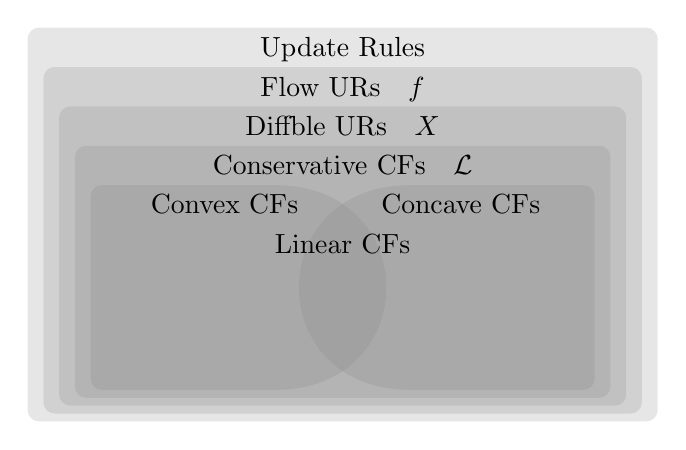
\begin{tikzpicture}
		\begin{scope}[fill=gray,fill opacity=0.2,rounded corners=4px]
			\fill (0,0) rectangle (8,5); % URs (Full Updates)
			\fill[] (0.2,0.1) rectangle (7.8,4.5); % Flow URs (Flows)
			\fill[] (0.4,0.2) rectangle (7.6,4.0); % Diffble URs (Vec Field)
			\fill[] (0.6,0.3) rectangle (7.4,3.5); % Conservative URs 
			\fill (0.8,0.4) -- (0.8, 3.0) -- (3, 3.0)
			 	to[out=0,in=0,looseness=2] (3,0.4) --cycle; % CONVEX
			\fill (7.2,0.4) -- (7.2, 3.0) -- (5, 3.0)
			 	to[out=180,in=180,looseness=2] (5,0.4) --cycle; % CONCAVE
		\end{scope}
		\begin{scope}[anchor=north]
			\node at (4.0, 5.0) {Update Rules};
			\node at (4.0, 4.5) {Flow URs~~~$f$};
			\node at (4.0, 4.0) {Diffble URs~~~$X$};
			% \node at (4.0, 3.5) {Conservative CFs~~~$\mathcal L$};
			\node at (4.0, 3.5) {Conservative CFs~~~$\mathcal L$};
			\node at (2.5, 3.0) {Convex CFs};
			\node at (4.0, 2.5) {Linear CFs};
			\node at (5.5, 3.0) {Concave CFs};
		\end{scope}
	\end{tikzpicture}
	\caption{%
		A map of different kinds of commitment functions and their representations.}
	\end{figure}
	}

\begin{figure*}
\centering
\begin{tikzpicture}
\begin{scope}[every node/.style={align=left,rounded corners=3,draw,thick,inner sep=5pt,anchor=center}]
	\node at (-5, 0) (fc) {Full-Confidence Update\\
		$(\,\cdot\mid \cdot\,) : \Theta \times \Phi \to \Theta$\\
			\small\hfill\color{gray}(idempotent)\hfill};
	\node at (0, -1.4)(flow) {Complete Positive Flows\\
		$f: [0,\infty] \times \Phi \times \Theta \to \Theta$\\
			\small\hfill\color{gray}(diffble, additive, limiting)\hfill};
	\node at (0, 1.4)(path) {Smoooth Paths\\ 
		$\gamma: [0,1] \times \Phi \times \Theta \to \Theta$\\
		\small\hfill\color{gray}(diffble, halting)\hfill};
	\node at (4.5, 0)(vfield) {Vector Fields \\
		$F : \Phi \to \mathfrak X(\Theta)$\\
		\small\hfill\color{gray}(complete, terminating)\hfill};
	\node at (8.5, 0) (loss) {Loss Repr \\
		$\mathcal L : \Theta \times \Phi \to \mathbb R$};
\end{scope}
	\draw[arr] (loss) to node[above]{$\hat\nabla$} (vfield);
%
	\draw[arr] (path) to[out=7,in=85] 
		node[right=5pt,pos=0.7]{$\frac{\partial}{\partial c}$} (vfield);
	\draw[arr] (flow) to[out=-7,in=-85]
		node[right=3pt,pos=0.7]{$\frac{\partial}{\partial t}$} (vfield);
%
	\draw[arr] (vfield) to[out=-95,in=-2] node[above=0pt,pos=0.75]
		% {$\int \mathrm dt$}
		% {$\int dt$} 
		{$\int$}
		(flow);
	% \draw[arr1] (vfield) to[out=90,in=0] node[below right]{$\int \mathrm dt$} (path);
	% \draw (vfield) to[out=90,in=0] node[above]{$\int \mathrm dt$} (flow);
	\draw[arr] (path) to node[above, sloped]{$c=1$} (fc);
	\draw[arr] (flow) to node[below,sloped]{$t=\infty$}(fc);
\end{tikzpicture}
\caption{Different representations of update functions, and the relationships they have with one another. 
Sections 3 and }\label{fig:map}
\end{figure*}



\commentout{
This general idea can be cleaned up by appeal to differential geometry.
Fix an input $\phi$.
Assuming that the update paths are differentiable in the degree of confidence at any initial beleifs, the collection of updates with infinitessimal confidence forms a complete vector field $X_\phi$ over the space of beliefs, whose integral curves are paths in belief space, parameterized by confidence $\beta \in [0,\infty]$.
% Of course, we may always convert this number back to $[0,1]$,
We step through this more carefully in \cref{sec:field-repr}.

%joe1*: NO!  This is not the place to bring up Reimannian metrics!
Finally, if our belief space is endowed with a Riemannian metric, so that we may take gradients, partial update functions may be specified by a loss.}


% natural measure of confidence that works in all cases,
% which 
% It turns out that there is a natural way of measuring confidence in all cases of interest, based on differential geometry of belief space. 
% Furthermore, in the case where belief states are Dempster-Shafer belief functions, 
% and inputs are simple support functions, this measure of confidence is what Shafer calls the ``weight of evidence''.
%% TODO: Shafer



% It is not always most natural for confidence to range between zero and one. 
% But there are many instances in which 
% However, there is a more universal representation of it in $[0, \infty]$

% While probability ranges from untenable (0) to undeniable (1),
% confidence ranges from completely untrustworthy $(\bot)$ to fully trusted ($\top$).




\commentout{
	\subsection{Other Conceptions of Confidence.}

	\textbf{Probability.}
	% Probability is a numerical scale that ranges from untenable (0) to undeniable (1).
	% No number on this scale is truly neutral.
	% One of the biggest shortcomings of probability is its inability to represent a truly neutral attitude towards a proposition.
	Some people do use ``confidence'' to mean the same thing as probability. When they say they have low confidence in $\phi$, they mean that they think $\phi$ is unlikely.

	One of the biggest shortcomings of probability is its inability to represent a truly neutral attitude towards a proposition.
	%  probability of $\frac12$ .
	% This shortcoming has perhaps been the primary selling point of many alternatives to probabiltiy, such as Dempster-Shafer Belief functions.
	A value of $\frac12$ may be equally far from zero as it is from one, but is by no means a neutral assessment in all cases: hearing that your favored candidate has a 50\% chance of winning is big news if a win was previously thought to be inevitable.
	For this reason, telling someone the odds are 50/50 is quite different from saying you have no idea.
	% By contrast, zero confidence represents a truly neutral stance; a statement with zero confidence has no effect.
	By contrast, zero confidence represents something truly neutral:
		a statement made with zero confidence does not stake out a claim, and
		a statement recieved with zero confidence does not affect the recipient's beliefs.
	Nevertheless, in some contexts, we will see that confidences correspond to to probabilities.

	\textit{Opacity.} To use a graphical metaphor, think of certainty as black or white.
	Probability describes shades of gray, while confidence describes opacity.
	If we are painting with black and start with a white canvas, there is a precise correspondence between the opacity and the resulting shade of gray.

	\textbf{Upper and Lower Probabilities.}
	Upper and lower probabilities can describe a neutral attitude towards a proposition, but they are not really a specification of trust, but rather a direct specification of a belief state.
	It isn't immediately clear how to use these representations of uncertainty to update, and they're a little too complex to function effectively as the primitive measure of trust that we're after.


	\textbf{Shafer's Weight of Evidence.}
	Shafer's ``weight of evidence'' is precisely the same concept we have in mind.
	Our analysis precsely reduces to his, in the setting where belief states are Belief functions (which generalize probabilities, but not, say, neural network weights), and observations are events.
	% This paper can be a generalization of Shafer's ``weight of evidence'' to a broader class of settings, where one might have very different belief states and observations.
	Thus, this paper can be viewed as generalizing this concept to a broader class of settings, without requiring that one adopt Shafer's conception of a belief state or an observation.


	\textbf{Variance and Entropy.}
	The inverse of variance, sometimes known as precision,
		is also commonly used to measure confidence.
	If a sensor is unreliable and can give a range of answers, the variance of the estimate is a very common way of quantifying this reliablility.
	If measurements have zero variance, in some sense one has absolute confidence ($\top$) in the sensor. If measurements have infinite variance, then in some sense one has no confidence in the sensor, since individual samples convey no information about the true value of the quantity measured.
	As with probability, inverse variance will coincide with confidence in some settings; we will see how in \cref{sec:variance}.

	Entropy, like variance, is a standard way of measuring uncertainty, and in some settings, confidence coincides with entropy (see \cref{sec:entropy}).
	The assumption underlying both approaches is that there's some ``true'' value of the variable, and that the randomness is epsistemic (due to sensor errors) rather than aleotoric (inherrent in the quantity being measured).

	\textbf{Confidence Intervals and Error Bars.}
	Another notion of the word ``confidence'' comes from the term ``confidence interval''.
	This concept arises in settings involving a probability distribution $\Pr(X)$ over a metric space $X$, typically $X = \mathbb R$.
	A 95\% confidence interval is the (largest) ball containing 95\% of the probability, and its size is a geometric measurement of how .
	This intuition behind this reading of the word confidence is the same as
}
